%   MSc Business Analytics Dissertation
%   Format based on skeleton template provided as part of module MIS40750
%
%   Title:     Optimising the design of buffer preparation in bioprocessing
%              facilities
%   Author:    Sean Tully
%
%   Chapter 3: Data
%
%   Change Control:
%   When     Who   Ver  What
%   -------  ----  ---  --------------------------------------------------------
%   06Jun16  ST    0.1  Begun 
%

\chapter{Data}\label{C.data}

\begin{quote}
Just as the largest library, badly arranged, is not so useful as a very
moderate one that is well arranged, so the greatest amount of knowledge, if not
elaborated by our own thoughts, is worth much less than a far smaller volume
that has been abundantly and repeatedly though over.  For only by universally
combining what we know, by comparing every truth with every other, do we fully
assimilate our own knowledge and get it into our power.

\hspace{2cm}--- Arthur Schopenhauer, \emph{On Thinking for Oneself}
\end{quote}

\section{Introduction}\label{S.intro3}

This section will outline what the input data might look like, including data
sources.
It will outline what form the output data and metrics should take.

For modeling a single process, a typical dataset consists of three distinct
files.
The first file is a table of data relating to the available selection of
vessels.
The second file is a table of data relating to parameters specific
to each buffer.
The third file comprises a collection of global parameters
that apply to all vessels and/or buffers.

One particular example, which is based on obfuscated data from a large-scale
facility, is used throughout this chapter to illustrate the format of the data.

\section{Vessel Data}\label{S.vesseldata}

A vessel dataset will contain entries for $M$ vessels ($M \in \mathbb{N}$).

Typically, when designing a large-scale production facility, buffer preparation
vessel volumes range from 1,000 l to 30,000 l.

When ordering such a vessel, the stated size of the vessel is usually a nominal
volume, which will differ from the liquid fill volume and may also differ from
the maximum working volume.
It is usual to round the stated or nominal volume to the nearest 1,000 l.

For the purposes of this study, it is assumed that, for each vessel $m \in M$,
the specified vessel volume, $V_{m}$ is the maximum working volume (in litres)
of the vessel, which is taken to be the maximum volume of buffer which can be
prepared in that vessel.

Vessels will also have a minimum working volume. 
It is usual to assume a minimum fill ratio of about 30\% of the vessel volume. 
This limitation arises due to the minimum agitation volume of the impeller in
the vessel. 
For the purposes of this simulation, the minimum fill ratio is a global
parameter.
It may be possible to specify a value of minimum fill ratio for every vessel
size, but this level of detail is typically neither required nor available.
As a result, the minimum fill ratio is dealt with in the parameters section.

For each vessel, $m \in M$, a (relative) cost, $c_{m}$, must also be defined.
Note that absolute costs are not required to find the vessel selection that
minimises costs.
Vessel costs tend not to scale linearly with volume.

Sample vessel data is given in \hyperref[tbl.vessel]{Table \ref*{tbl.vessel}}.
In this dataset, the cost datum for each vessel size has been estimated by
raising the vessel volume (in litres) to a power of 0.6 and rounding to two
decimal places.
Note that the vessel volumes, $V_{m}$, are larger than the nominal volumes
indicated in the `names' column.  The contents of the `names' column are
treated as identifiers and are not used in any calculation.
\begin{table}[h!]
    \centering
    \caption{Vessel data for large-scale example}
    \label{tbl.vessel}
    \begin{tabular}{l | r | r}
        names & volumes & costs\\
        & $V_{m}$ (l) & $c_{m}$ (--)\\\hline
        2000 l & 2222.0 & 95.64\\
        4000 l & 4444.0 & 144.96\\
        5000 l & 5556.0 & 165.72\\
        8000 l & 8889.0 & 219.71\\
        10000 l & 11111.0 & 251.19\\
        12000 l & 13333.0 & 280.23\\
        15000 l & 16667.0 & 320.37\\
        20000 l & 22222.0 & 380.73\\
        25000 l & 27778.0 & 435.28\\
    \end{tabular}
\end{table}

\section{Buffer Data}\label{S.bufferdata}

A buffer dataset will contain entries for $N$ buffers ($N \in \mathbb{N}$).
For each buffer, $n \in N$, the dataset will contain, at a minimum, its
required preparation volume (in litres), $U_{m}$.

If nothing was known about the scheduling of the prodcution process, a simple
simulation could be carried out without scheduling.
Such a simulation would assume a fixed duration for all operations in the 
preparation procedure and would require knowledge of the cycle time and an
additional parameter representing the maximum utilisation ratio of the
preparation vessels (see \hyperref[S.parameters]{Section \ref*{S.parameters}}).

For a complete model, with scheduling, we also need to know when each buffer
is first required by the process, and the duration for which it is required.

For each buffer, $n \in N$, its time of first use, $t_{USE,n}$, is the time
when the process draws the first drop of buffer from its hold vessel.
This time is relative to some batch datum, e.g. the start of the batch or the
start of downstream processing.
The choice of datum is unimportant once it is consistently used.

For each buffer, $n \in N$, its duration of first use, $\Delta t_{USE,n}$, is
the duration from when the process draws the first drop of buffer from its hold
vessel to when it finishes drawing the last drop of buffer from the same
vessel.
Note that a process may draw buffer discontinuously from a hold vessel, e.g. a
cleaning buffer may be drawn from its hold vessel for a few minutes at the end
of a chromatography procedure and may not be required again until near the end
of another chromatography procedure a day or two later, but may not be required
at all in the intervening period.
Note the use of the general convention that \emph{durations} are denoted by
$\Delta t$, whereas \emph{times} (relative to some datum) are denoted by $t$.
It is assumed that all times and durations are in hours.

For each buffer, $n$, $\Delta t_{USE,n}$ must be sufficiently less than
the cycle time so that there is opportunity to \emph{turn around} its hold
vessel (i.e. sufficient time must exist after use of the buffer to clean and
sterilise the vessel, receive the subsequent batch of buffer and hold for a 
sufficient duration before use of that buffer is required by the subsequent
batch).

Sample buffer data is given in \hyperref[tbl.buffer]{Table \ref*{tbl.buffer}}.

\begin{table}[h!]
    \centering
    \caption{Buffer data for large-scale example}
    \label{tbl.buffer}
    \begin{tabular}{l | c | c | c}
        names & required volumes & use start times & use durations\\
        & $U_{n}$ (l) & $t_{USE,n}$ (h) & $\Delta t_{USE,n}$ (h)\\ \hline
        \text{Buffer \#1} & 19676.0 & 733.87 & 48.99\\
        \text{Buffer \#2} & 18528.0 & 644.18 & 36.95\\
        \text{Buffer \#3} & 17346.0 & 684.60 & 49.27\\
        \text{Buffer \#4} & 15055.0 & 764.96 & 28.01\\
        \text{Buffer \#5} & 13896.0 & 628.54 & 52.59\\
        \text{Buffer \#6} & 10267.0 & 728.99 & 53.12\\
        \text{Buffer \#7} & 10070.0 & 677.94 & 20.86\\
        \text{Buffer \#8} & 6797.0 & 728.99 & 53.12\\
        \text{Buffer \#9} & 6716.0 & 612.90 & 70.40\\
        \text{Buffer \#10} & 4632.0 & 645.50 & 35.63\\
        \text{Buffer \#11} & 3780.0 & 729.34 & 43.19\\
        \text{Buffer \#12} & 3694.0 & 678.92 & 42.17\\
    \end{tabular}
\end{table}

\section{Parameters}\label{S.parameters}

In addition to the buffer-specific and vessel-specific data detailed above,
some global parameters are required to specify the problem.
For the large-scale example, these parameters are tabulated in
\hyperref[tbl.parameters]{Table \ref*{tbl.parameters}} and are described in
more detail hereafter.
\begin{table}[h!]
    \centering
    \caption{Global parameters for large-scale example}
    \label{tbl.parameters}
    \begin{tabular}{l | l | c | c}
        symbol & short description & value & unit\\ \hline
        $\lambda$ & process cycle time & 96.0 & h\\
        $\Delta t_{PREP,PRE}$ & prep pre duration & 11.0 & h\\
        $\Delta t_{PREP,POST}$ & prep post duration & 2.5 & h\\
        $\Delta t_{TRANSFER}$ & transfer duration & 2.2 & h\\
        $\Delta t_{HOLD,PRE}$ & hold pre duration & 9.0 & h\\
        $\Delta t_{HOLD,POST}$ & hold post duration & 1.0 & h\\
        $\Delta t_{HOLD,MIN}$ & minimum hold duration & 12.0 & h\\
        $\Delta t_{HOLD,MAX}$ & maximum hold duration & 60.0 & h\\
        $r_{MINFILL}$ & minimum fill ratio & 0.27 & --\\
        $r_{UTIL}$ & maximum utilisation ratio & 0.7 & --\\
    \end{tabular}
\end{table}

%TODO
\textbf{TODO: Describe parameters}

\section{Output Data}\label{S.outputdata}

\begin{figure}
    \centering
    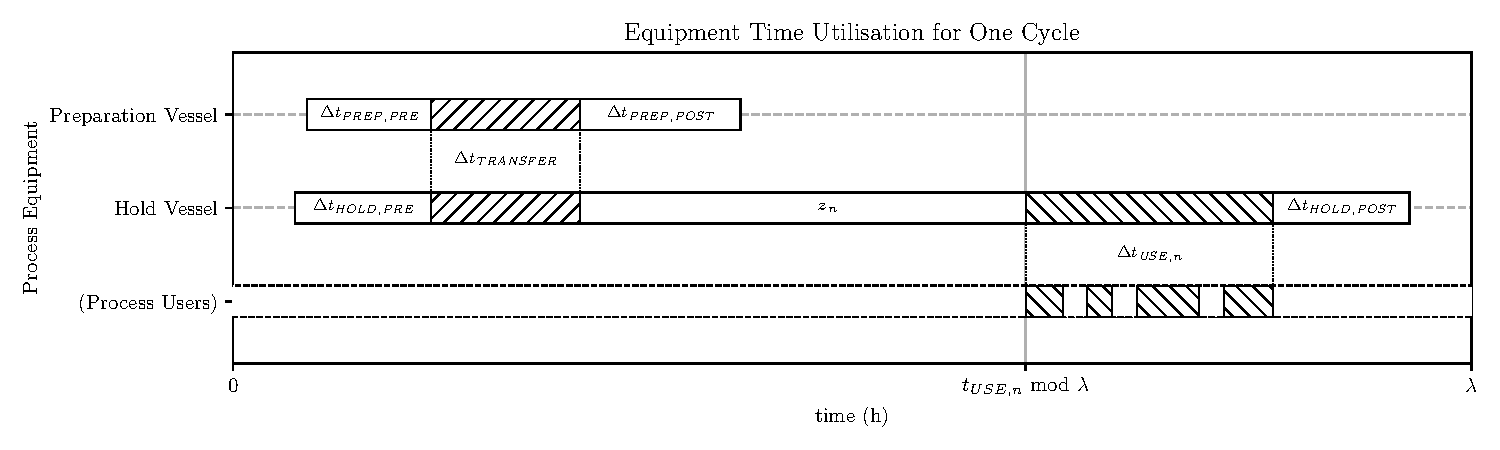
\includegraphics[angle=0,scale=0.55]{./figures/explanatory.pdf}
    \caption{Equipment Time Utilisation for a Single Buffer}
    \label{fig.explanatory}
\end{figure}
